\documentclass[12pt]{article}
\usepackage{graphicx}
\usepackage{parskip}
\usepackage{multicol}
\usepackage{csquotes}
\setlength{\parindent}{15pt}
\setlength{\parskip}{15pt}
\graphicspath{ {./} }


\begin{document}
\begin{center}
\section*{American Sign Language with Convolutional Neural Networks}

Addison Boyer \\
Machine Learning, Fall 2019 \\


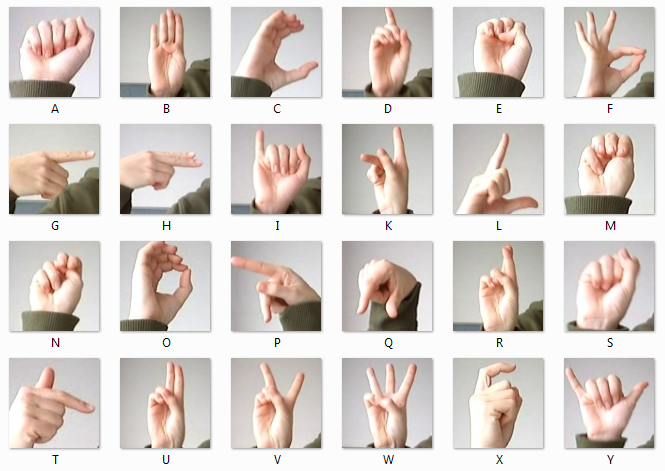
\includegraphics[scale=.75]{amer_sign2}
\end{center}

\pagebreak

\begin{multicols}{2}
\subsection*{Introduction}
The National Institute on Deafness and Other Communication Disorders (NIDCD) defines American Sign Language (ASL) as 
\enquote{a complete, natural language that has the same linguistic properties as spoken languages, with grammar that differs from English.}



\subsection*{Methods}

Methods go here.

\subsection*{Results}

Results go here.


\subsection*{Discussion}

Discussion goes here.

\subsection*{Conclusion}

Conclusion goes here.

\end{multicols}

\subsection*{References}

References go here.


\end{document}